\documentclass[12pt,a4j]{jarticle}
\usepackage{graphicx}
\begin{document}
\title{コンピュータリテラシレポート#12}
\author{2120029, 政野玄空}
\date{7月2日}
\maketitle


\section{課題の再掲}
\begin{itemize}
  \item 演習2 a h1\verb|~|h6の見出し要素から1つ以上選び、自分がかっこいいと思うデザインになるようCSSで工夫をする
  \item 演習3 じぶんの作成したWebページに関する説明を行うLaTeX文章を作成する。a id機能またはclass機能を使って「特定のなにかだけ表現が違う」ようにしてみる。
\end{itemize}

\section{レポートの本文}

まずはじめにh1、h2の場所をそれぞれ変更した。一番大きい見出しは真ん中、次に大きいのは左によるようにした。
色も変えてみたがよみにくいのでやめた。
bodyのbackground-imgに適当に拾った画像を入れた。

次に演習3aのidをあてて一部だけ違うようにするだが、あまりガイドを見ずにすすめていたためかなりわかりにくい。
まず全体をwrapというidを当てたdivで囲みwidth: 100\verb|%|;height: 100\verb|%|;overflow: hidden;を設定した。
widthを小さくしたりすれば特定のなにかだけ表現が違うに当てはまる気がするがしたい意思がないのでやらない。
contentsというidにはposition relativeが設定されている。

%(作成したWebページの図を入れる)
\begin{center}
  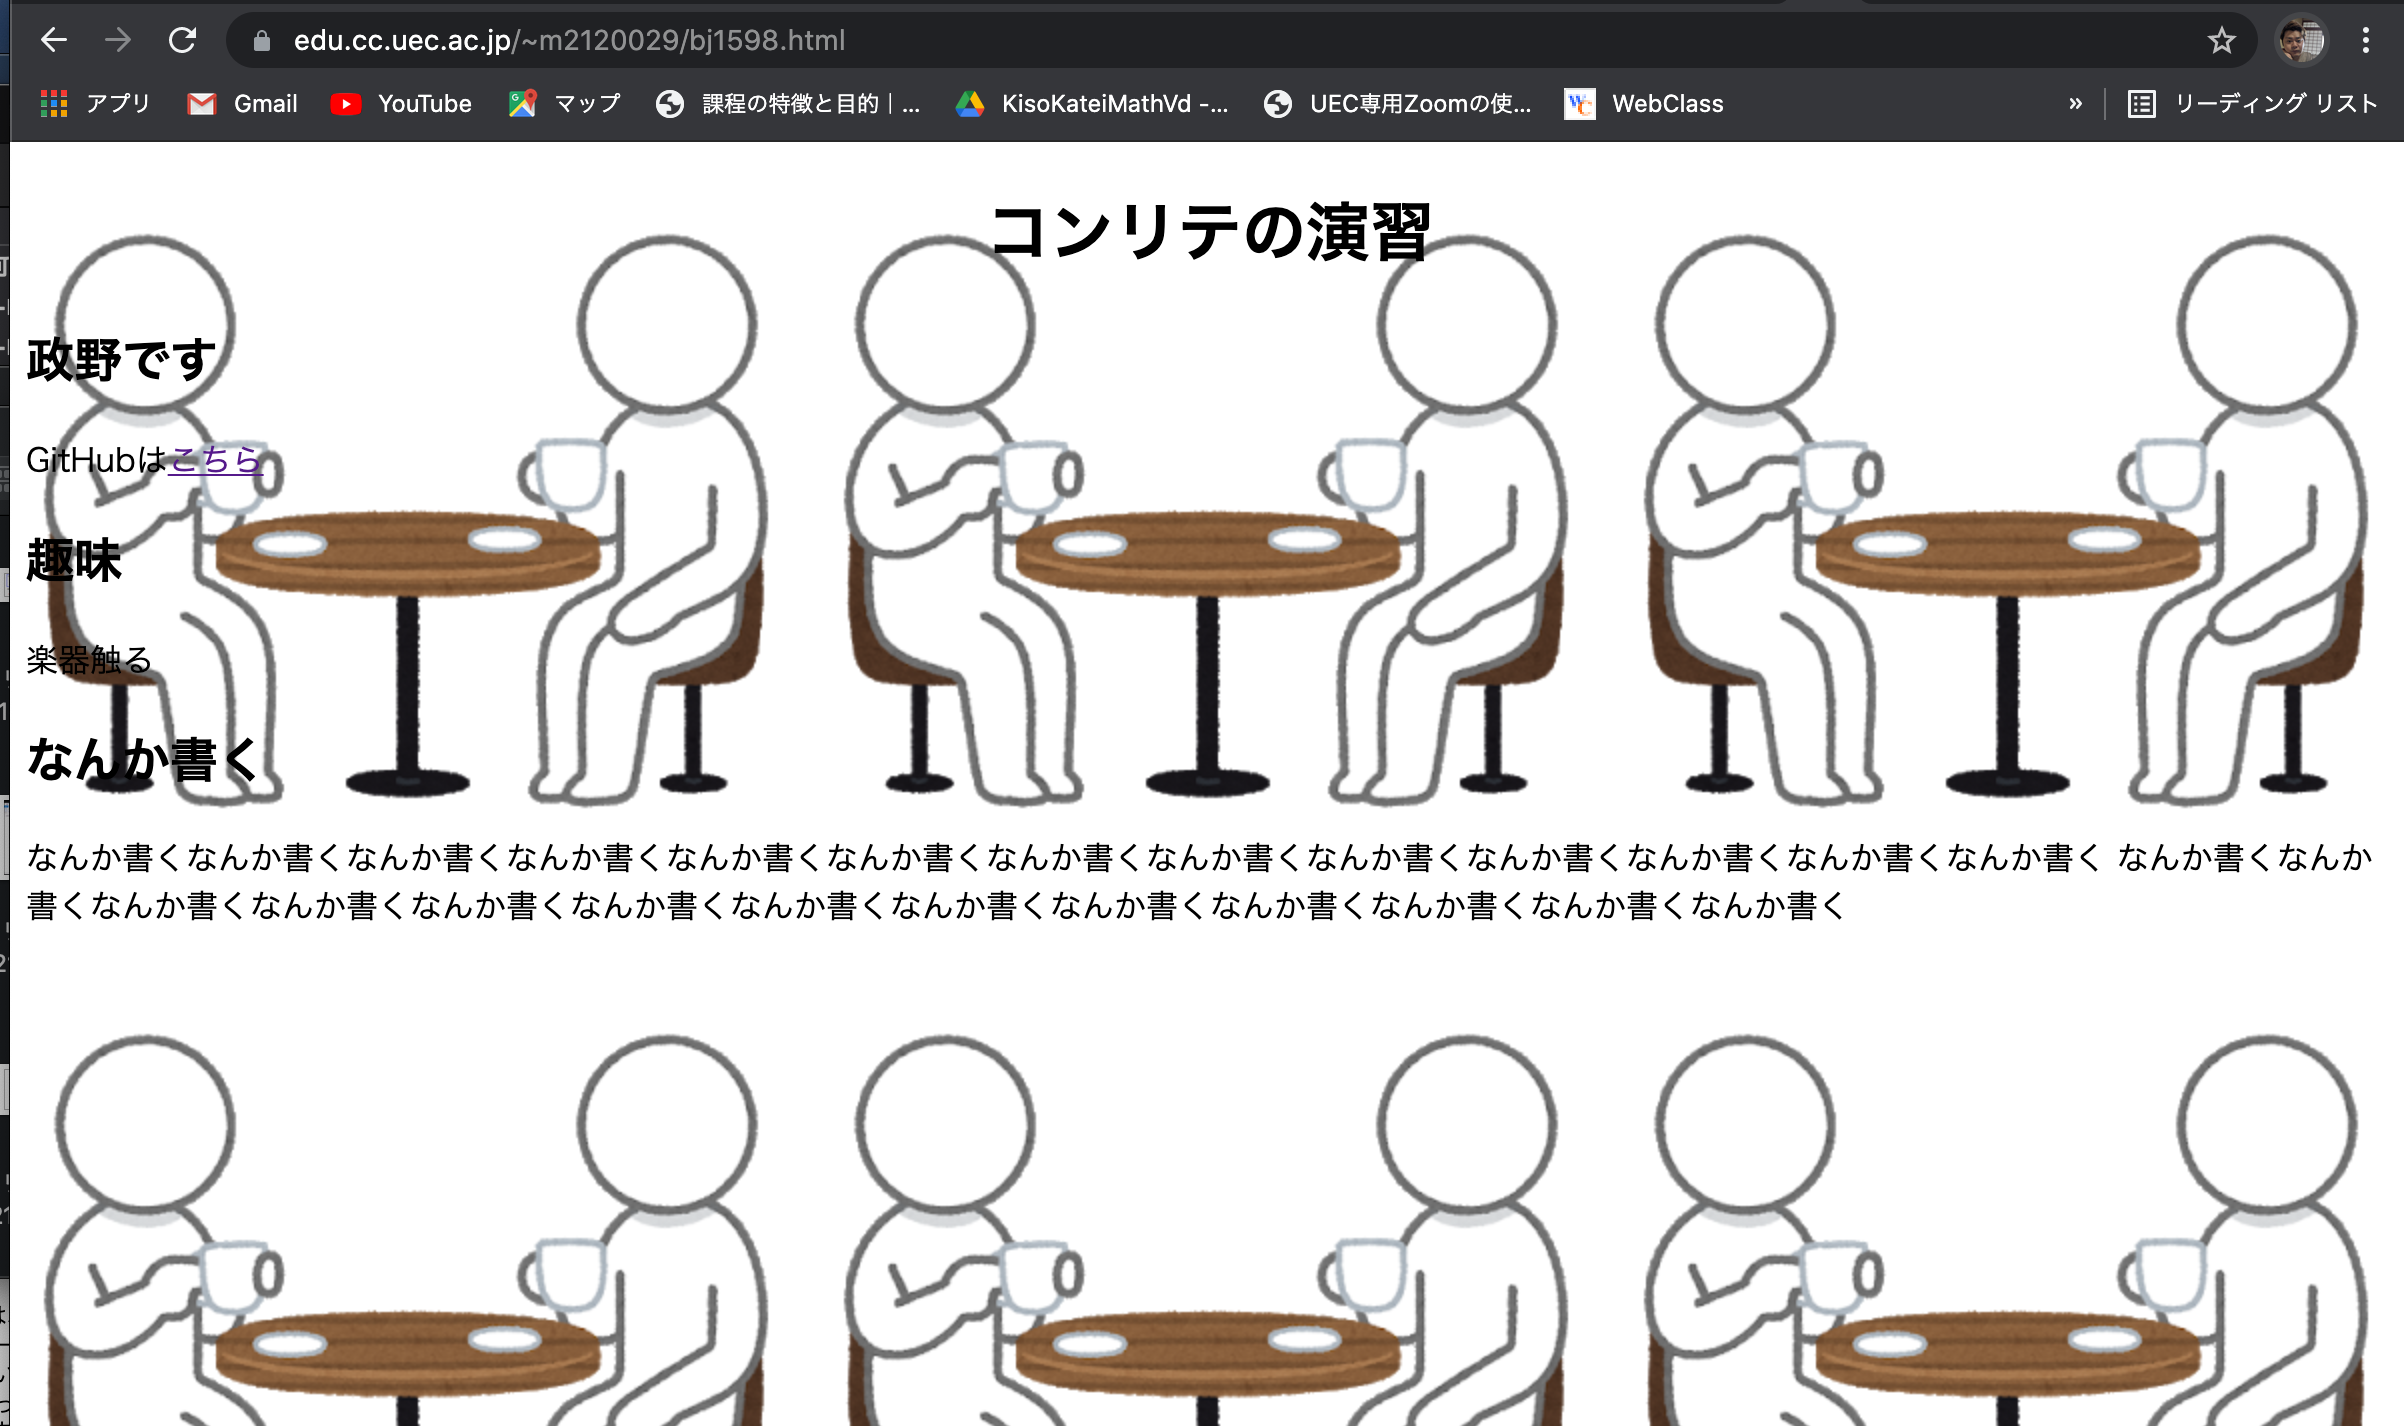
\includegraphics[width=12cm]{scst.eps}
\end{center}

%(読み手が確認できるようURLも載せる。 ~ の表現に注意)

https://www.edu.cc.uec.ac.jp/\verb|~|m2120029/bj1598.html

\section{考察}
( ここに考察を記入 )
さすがにもう少しまともなページを作りたかったが時間の兼ね合いもありかなり残念な結果になった。
きれいでシンプルなページをなるべくはやく完成させることができる能力を鍛えたい。
あまりフロントエンドの仕事はしないので気になったときしか開発者モードで見ることがなかったが、きれいだと思うサイトは積極的に構成を見に行くことにしたい。
また無料のテンプレートを使う手もあったがあまり意味がないのでやめた。
ブロック要素の中で、Flexboxの登場によって現代ではtableはほとんど見なくなったように思う。
\section{アンケート}

\subsection{Q1:HTMLによるページの記述はどれくらい知っていましたか。今回やってみてどうでしたか。}
( ここにQ1の回答を記入 )
最低限は知っているがきれいに作るのが難しかった。
\subsection{Q2:CSSによる表現の指定はどれくらい知っていましたか。今回やってみてどうでしたか。}
( ここにQ2の回答を記入 )
ある程度知っているが一番難しいと思っている。
\subsection{Q3:リフレクション (今回の課題で分かったこと)・感想・要望をどうぞ。}
( ここにQ3の回答を記入 )
とてもhtml/cssが苦手なことがわかった。
\end{document}
